\section{Conjugate gradient}\label{sec:conjugate_gradient}
In this section we will talk about the conjugate gradient method in the same way we did for L-BFGS and thin QR, by first introducing the algorithm itself and then by analyzing its complexity and the performances obtained by applying to our case. 

\subsection{Overview on conjugate gradient}
The conjugate gradient is an iterative algorithm for solving linear systems of equations
\begin{equation}
    Ax=b
    \label{eq:cg_linear_system}
\end{equation}
where $A \in \mathbb{R}^{n\times n}$ is a symmetric positive definite matrix \footnote{$X=X^T$ and $zAz^T>0$ $\forall z \neq 0 \in \mathbb{R}^{n}$} and $x,b \in \mathbb{R}^{n}$, where $x$ is called as the unique solution. Since $A$ is symmetric positive definite, then \eqref{eq:cg_linear_system} can be stated as a minimization problem (a strictly convex one to be more precise)
\begin{subequations}
    \begin{equation}
        min\hspace{1mm} \phi(x) \stackrel{def}{=} \frac{1}{2}x^TAx - b^Tx
        \label{eq:cg_minimization_function}
    \end{equation}
    \begin{equation}
        \nabla \phi(x) = Ax-b \stackrel{def}{=} r(x)
        \label{eq:cg_minimization_gradient}
    \end{equation}
    \label{eq:cg_minimization}
\end{subequations}

\noindent In short, minimizing \eqref{eq:cg_minimization_function} means that we need to solve either \eqref{eq:cg_minimization_gradient} (with $r(x)=0$) or \eqref{eq:cg_linear_system}.

\subsubsection{Conjugate direction methods}
\noindent As the name suggests the conjugate gradient method exploits a property called \textit{conjugacy} to generate a set of vectors. A set of non-zero vectors $\{ p_0, p_1 \dots p_l\}$ is known as \textit{conjugate} of a symmetric definite positive matrix $A$ if
\begin{equation}
    p_i^TAp_j=0, \hspace{3mm} \forall i\neq j
    \label{eq:cg_conjugacy}
\end{equation}

\noindent \eqref{eq:cg_conjugacy} is vital to minimize \eqref{eq:cg_minimization_function} in, at maximum, $n$ steps, but first we need to consider the \textit{conjugate direction} method. Given a starting point $x_0 \in \mathbb{R}^n$ a a set of conjugate directions $\{ p_0, p_1 \dots p_{n-1}\}$, the sequence $\{ x_k\}$ is generated step by step by
\begin{equation}
    x_{k+1} = x_k + \alpha_kp_k
    \label{eq:cg_step}
\end{equation}

\noindent \eqref{eq:cg_step} seems identical to what we have seen for the L-BFGS in \eqref{eq:bfgs_step} and also the step size $\alpha$ will be similar, which is now defined as
\begin{equation}
    \alpha_k = -\frac{r_k^Tp_k}{p_k^TAp_k}
    \label{eq:cg_alpha}
\end{equation}

\noindent We now have enough tools for theorem \ref{theorem:cg_conjugate_direction} (theorem 5.1 from \cite{nocedal1999numerical}, the proof can also be found there).
\begin{theorem}
    For any $x_0 \in \mathbb{R}^n$ the sequence $\{ x_k\}$ generated by the conjugate direction algorithm \eqref{eq:cg_step}, then \eqref{eq:cg_alpha} converges to the solution $x^*$ of the linear system \eqref{eq:cg_linear_system} in at most $n$ steps.
    \label{theorem:cg_conjugate_direction}
\end{theorem}

\noindent Theorem \ref{theorem:cg_conjugate_direction} tell us some properties of conjugate directions:
\begin{enumerate}
    \item If $A$ is diagonal, then the contours of \eqref{eq:cg_minimization_function} are ellipses whose axes are aligned with the coordinate directions, therefore, we can find the minimum by performing one-dimensional minimizations along the coordinate directions $e_1, e_2, \dots e_n$. If $A$ is not diagonal we need to precondition it in order to obtain the same behaviour.
    \item When the Hessian is diagonal, each coordinate minimization determines one of the components of the solution $x^*$.
\end{enumerate}

\noindent The second property holds even when the Hessian is not diagonal and this is proven by theorem \ref{theorem:expanding_subspace_minimization} (theorem 5.2 and proof from \cite{nocedal1999numerical}).
\begin{theorem}
    Let $x_0 \in \mathbb{R}^n$ be any starting point and suppose that the sequence $\{ xk \}$ is generated by the conjugate direction algorithm \eqref{eq:cg_step}, \eqref{eq:cg_alpha}. Then
    \begin{equation}
        r_k^Tp_i = 0 \hspace{3mm} for \hspace{1mm} i=0,...k-1
        \label{eq:cg_residual_direction}
    \end{equation}
    and $x_k$ is the minimizer of \eqref{eq:cg_minimization_function} over the set
    \begin{equation}
        \{x | x = x_0 +span\{ p_0, p_1,\dots, p_{k-1}\} \}
    \end{equation}
    \label{theorem:expanding_subspace_minimization}
\end{theorem}

\subsubsection{Conjugate gradient method}
As the name suggest, the conjugate gradient method is a conjugate direction method with the very nice fact that to compute a new vector $p_k$ based only on $p_{k-1}$, hence it does not need the entire conjugate set. This implies that the method requires little storage and computations.
\vspace{3mm}

\noindent In the conjugate gradient method, each direction $p_k$ is chosen to be a linear combination of the negative residual $-rk$ (which, by \eqref{eq:cg_minimization_gradient} is the steepest direction for \eqref{eq:cg_minimization_function}) and the previous direction $p_{k-1}$, formally
\begin{equation}
    p_k = -r_k + \beta_kp_{k-1}
    \label{eq:cg_direction}
\end{equation}

\noindent where $\beta_k$ is a value determined by the requirement that $p_k$ and $p_{k_1}$ must be conjugate with respect to $A$, moreover, by doing the product of \eqref{eq:cg_direction} with $p^T_{k-1}A$ and imposing the condition that $p^T_{k-1}Ap_k=0$, we find that
\begin{equation}
    \beta_k = \frac{r^T_kAp_{k-1}}{p^T_{k-1}Ap_{k-1}}
    \label{eq:cg_beta}
\end{equation}

\noindent We need to show that the directions $p_0, p_1,\dots, p_{n-1}$ are indeed conjugate, which by theorem \ref{theorem:cg_conjugate_direction} implies that the method terminates in $n$ steps. Theorem \ref{theorem:cg_krylov} (theorem 5.3 from \cite{nocedal1999numerical}) establishes this property and two other important properties:
\begin{enumerate}
    \item The residuals $r_i$ are mutually orthogonal.
    \item Each search direction $p_k$ and residual $r_k$ is contained in the \textit{Krylov subspace of degree $k$ for $r_0$}, defined as
    \begin{equation}
        K(r_0, k) \stackrel{def}{\approx} span\{ r_0, Ar_0, \dots, A^kr_0 \}
        \label{eq:cg_krylov_subspace}
    \end{equation}
\end{enumerate}

\begin{theorem}
Suppose that the k-th iterate generated by the conjugate gradient method is not the solution point $x^*$. The following four properties hold
    \begin{subequations}
        \begin{equation}
            r_k^Tr_i = 0, \hspace{3mm} for\hspace{1mm} i=0,\dots, k-1
        \end{equation}
        \begin{equation}
            span\{ r_0,r_1,\dots,r_k \} = span\{ r_0, Ar_0,\dots, A^kr_0\}
        \end{equation}
        \begin{equation}
            span\{ p_0,p_1,\dots,p_k \} = span\{ r_0, Ar_0,\dots, A^kr_0\}
            \label{eq:cg_krylov_property}
        \end{equation}
        \begin{equation}
            p^T_kAp_i = 0, \hspace{3mm} for\hspace{1mm} i=0, \dots, k-1
        \end{equation}
    \end{subequations}
    \label{theorem:cg_krylov}
\end{theorem}

\noindent The proof of theorem \ref{theorem:cg_krylov} can be found after theorem 5.3 from \cite{nocedal1999numerical}. As last thing for this part, we can rewrite \eqref{eq:cg_alpha} by using \eqref{eq:cg_direction} and \eqref{eq:cg_residual_direction} to obtain
\begin{equation}
    \alpha_k = -\frac{r_k^Tp_k}{p_k^TAp_k} = -\frac{r_k^T(-r_k+\beta_kp_{k-1})}{p_k^TAp_k} = \frac{r_k^Tr_k}{p_k^TAp_k}
    \label{eq:cg_alpha_efficient}
\end{equation}

\noindent Moreover, noting the relation between \eqref{eq:cg_step}, and the k-th residual $r_k=Ax_k-b$, we can write
\begin{equation}
    r_{k+1} = rk+\alpha_kAp_k
    \label{eq:cg_residual}
\end{equation}

\noindent We can also rewrite \eqref{eq:cg_beta} based, again, on \eqref{eq:cg_direction}, \eqref{eq:cg_residual_direction} and \eqref{eq:cg_residual}
\begin{equation}
    \beta_k = \frac{r^T_kAp_{k-1}}{p^T_{k-1}Ap_{k-1}} = \frac{r^T_k\frac{r_k-r_{k-1}}{\alpha_{k-1}}}{p^T_{k-1}\frac{r_k-r_{k-1}}{\alpha_{k-1}}} = \frac{r^T_k(r_k-r_{k-1})}{p^T_{k-1}(r_k-r_{k-1})} = -\frac{r^T_kr_k}{r^T_{k-1}p_{k-1}} = \frac{r^T_kr_k}{r^T_{k-1}r_{k-1}}
    \label{eq:cg_beta_efficient}
\end{equation}

\noindent We now have everything needed to build the conjugate gradient algorithm and to apply to our case.

\subsection{Solving LLS with conjugate gradient}\label{subsec:solve_LLS_cg}
Diving into our lls problem we first notice that $\hat{X}$ is not symmetric positive definite, hence we can not apply the conjugate gradient method in a straightforward way. But, as we have seen in \ref{subsec:introduction_lls}, the solution to the lls problem is obtained by solving \eqref{eq:normal_equation} and, luckily for us, $\hat{X}^T\hat{X}$ is symmetric positive definite (this is also the Hessian of the lls which we have shown to be positive definite in \ref{subsec:introduction_convexity}), so we can apply that to our case.
\vspace{3mm}

\noindent The optimal solution $w_*$, therefore, can be found in the following way
\begin{equation}
    w^T_*\hat{X}^T\hat{X}=\hat{y}^T\hat{X} \Longleftrightarrow \hat{X}^T\hat{X}w_*=\hat{X}^T\hat{y}
    \label{eq:cg_solving_normal_equation}
\end{equation}

\noindent $\hat{X}^T\hat{X} \in \mathbb{R}^{n \times n}$ has full column rank, therefore is symmetric positive definite and we can now solve the lls with the conjugate gradient, but, before we proceed further, we should rewrite \eqref{eq:cg_solving_normal_equation} in a more readable way
\begin{equation}
    \hat{X}^T\hat{X}w_*=\hat{X}^T\hat{y} \Longleftrightarrow Aw_*=b
    \label{eq:cg_normal_equation_rewritten}
\end{equation}

\noindent From now on we will refer to the right side of \eqref{eq:cg_normal_equation_rewritten} over the next sections. We now have everything needed to show the conjugate gradient method in \autoref{algorithm:cg}

\begin{algorithm}[H]
    \caption{Conjugate gradient}
    \label{algorithm:cg}
    Given $x_0 \in R^m$;\\
    $r_0=Ax_0-b$;\\
    $p_0=-r_0$;\\
    $k=0$;\\
    \While{$r_k\neq 0$} {
        $\alpha_k =  \frac{r_k^Tr_k}{p_k^TAp_k}$;\\
        $x_{k+1} = x_k + \alpha_kp_k$;\\
        $r_{k+1} = r_k + \alpha_kAp_k$;\\
        $\beta_{k+1} = \frac{r^T_{k+1}r_{k+1}}{r^T_kr_k}$;\\
        $p_{k+1}=-r_{k+1}+\beta_{k+1}p_k$;\\
        $k=k+1$;\\
    }
    \Return{$x_{k+1}$};
\end{algorithm}

\noindent Of course, we can improve \autoref{algorithm:cg} by computing $Ap_k$, $r^T_kr_k$ before $\alpha_k$ and $\beta_{k+1}$ in order to obtain a better execution time.
\vspace{3mm}

\noindent Moreover, in order to apply the conjugate gradient algorithm to solve the lls problem, we need to compute the matrix product $A = \hat{X^T}\hat{X}$, as we can see from \eqref{eq:cg_normal_equation_rewritten}. Therefore, the resulting matrix has a conditioning number $\kappa(A) = \kappa(\hat{X})^2$ and this implies that $A$ is extremely ill-conditioned when $\lambda$ is small (recall the conditioning number of our matrices $\hat{X}$ from \autoref{tab:condition_number}). This issue can be mitigated by avoiding to form the matrix $A$ explicitly, because it is less sparse than $\hat{X}$.
\vspace{3mm}

\noindent By looking at \autoref{algorithm:cg}, we can compute $r_0$ by first finding the product $\hat{X}x_{0}$, and then $\hat{X^T}\hat{X}x_{0}$. Also, the update of $\alpha_k$ should be modified as following
\begin{equation}
    \alpha_k =  \frac{r_k^Tr_k}{(\hat{X}p_k)^{T}\hat{X}p_k}
    \label{eq:cg_rewritten_alpha}
\end{equation}
knowing that the inner product $\langle p, \hat{X}^T \hat{X} p \rangle = \langle \hat{X}p, \hat{X}p \rangle$.
\vspace{3mm}

\noindent Finally, we modify the update of $r_k$ with
\begin{equation}
    r_{k+1} = r_k + \alpha_k \hat{X}^T (\hat{X} p_k)
\end{equation}
This normal equations approach was suggested by Björck and Elfving \cite{bjorck1979accelerated}, and it allowed us to reach a solution that is an order of magnitude better than our original approach.

\subsection{Convergence and complexity}
From \autoref{theorem:cg_conjugate_direction} we know that conjugate gradient converges at the solution in at most $n$ steps, this can be improved when the distribution of the eigenvalues of $A$ has certain features. First, we can notice that at each step of the conjugate gradient method, the error term $e_{k+1}=w_{k+1}-w^*$ can be rewritten as
\begin{equation}
    e_{k+1} = e_0 + span\{r_0,Ar_0,A^2r_0,\dots,A^kr_0\} = e_0 + span\{Ae_0,A^2e_0,\dots,A^ke_0\}
    \label{eq:cg_error_subspace}
\end{equation}
then by considering a polynomial $P_k(A)$ of degree $k$, we can state that the error term assumes the following form
\begin{equation}
    e_{k+1} = w_{k+1}-w^* = P_k(A)(w_0-w^*) = P_k(A)e_0 = \left( I+\sum_{i=1}^k \gamma_iA^i \right)e_0
    \label{eq:cg_wk+1_and_wstar}
\end{equation}
for some constants $\gamma_i$ related to $\beta_i$ and $\alpha_i$ (this fact is not important for the pursuance of this section). What is interesting to us is the fact that the algorithm chooses each $\gamma_i$ in order to minimize
\begin{equation}
    \lVert e_{k+1}\rVert_A^2 = e_{k+1}^TAe_{k+1} = (w_{k+1}-w^*)^TA(w_{k+1}-w^*)
    \label{eq:cg_weighted_norm_c}
\end{equation}

\noindent Moving now forward on our analysis, let $0<\theta_1\leq\dots\leq\theta_m$ be the eigenvalues of $A$ and let $v_1,\dots, v_n$ be the corresponding orthonormal eigenvectors, such that
\begin{equation}
    A=\sum^m_{i=1}\theta_iv_iv^T_i
    \label{eq:cg_rewritten_matrix}
\end{equation}
then, we can rewrite $e_0$ as
\begin{equation}
    e_0=w_0-w^*=\sum_{i=1}^n\xi_i v_i
    \label{eq:cg_w0_wstar}
\end{equation}
for some coefficient $\xi_i$. Moreover, $P_k$ can take either a scalar or a matrix as argument and the results will be the same, so it can be shown that
\begin{equation}
    P_k(A)v_i=P_k(\theta_i)v_i \hspace{3mm} \forall i=1,\dots,m
\end{equation}

\noindent Therefore, by plugging \eqref{eq:cg_w0_wstar} into \eqref{eq:cg_wk+1_and_wstar} we obtain that
\begin{equation}
    e_{k+1}=w_{k+1}-w^*=\sum_{i=1}^n\xi_i P_k(\theta_i)v_i
    \label{eq:cg_rewritten_xk+1_and_xstar}
\end{equation}

\noindent By looking at \eqref{eq:cg_weighted_norm_c}, we can also rewrite \eqref{eq:cg_rewritten_xk+1_and_xstar} as
\begin{equation}
    \lVert e_{k+1}\rVert_A^2=\lVert w_{k+1}-w^*\rVert^2_A=\sum_{i=1}^n\xi_i^2[P_k(\theta_i)]^2\theta_i
\end{equation}

\noindent Then, by extracting the largest of the terms $[P_k(\theta_i)]^2$ we retrieve that
\begin{equation}
     \lVert w_{k+1}-w^*\rVert^2_A\leq \min_{P_k} \max_{1\leq i\leq n}[P_k(\theta_i)]^2(\sum_{j}^n\theta_j\xi^2_j)=\min_{P_k} \max_{1\leq i\leq n}[P_k(\theta_i)]^2\lVert w_0-w^*\rVert_A^2
     \label{eq:cg_upper_bound}
\end{equation}

\noindent \eqref{eq:cg_upper_bound} gives us an upper bound, allowing us to estimate the convergence rate of the method by estimating
\begin{equation}
    \min_{P_k} \max_{1\leq i\leq n}[P_k(\theta_i)]^2
    \label{eq:cg_upper_bound_quantity}
\end{equation}
In short, we need to look for a $P_k$ that minimizes \eqref{eq:cg_upper_bound_quantity}.
\vspace{3mm}

\noindent Following what we have seen in this section until now, we can introduce \autoref{theorem:cg_eigenvalues} and Theorem \ref{theorem:cg_eigenvalues_estimate} (theorems 5.4 and 5.5 from \cite{nocedal1999numerical}, their proofs are also there).
\begin{theorem}
    If A has only $r$ distinct eigenvalues, then the CG iteration will terminate at the solution in at most $r$ iterations.
    \label{theorem:cg_eigenvalues}
\end{theorem}
Following the same reasoning, Leunberger derived an estimate
\begin{theorem}
    If $A$ has eigenvalues $\theta_1\leq\dots\leq\theta_n$, we have that
    \begin{equation}
        \lVert w_{k+1}-w^*\rVert_A^2\leq \left(\frac{\theta_{n-k}-\theta_1}{\theta_{n-k}+\theta_1}\right)^2\lVert w_0-w^*\rVert_A^2
    \end{equation}
    \label{theorem:cg_eigenvalues_estimate}
\end{theorem}
By defining $\epsilon=\theta_{n-j}-\theta_1$, Theorem \ref{theorem:cg_eigenvalues_estimate} tells us that after $j+1$ steps of applying the method, we obtain
\begin{equation}
    \lVert e_j\rVert_A\approx\epsilon\lVert e_0\rVert_A
    \label{eq:cg_epsilon}
\end{equation}
Another last thing is the fact that $\epsilon$ from \eqref{eq:cg_epsilon} can be rewritten in terms of $\kappa(A)=\frac{\theta_m}{\theta_1}$, giving us the following
\begin{equation}
    \lVert e_j \rVert_A=\lVert w_{j}-w^*\rVert_A\approx2\left(\frac{\sqrt{\kappa(A)}-1}{\sqrt{\kappa(A)}+1}\right)^j\lVert e_0\rVert_A
    \label{eq:cg_rewritten_epsilon}
\end{equation}
The bound from \eqref{eq:cg_rewritten_epsilon} is a large overestimation of the error, but it could be useful when the only information we know about $A$ are its maximum and minimum eigenvalues.

\paragraph{Complexity}
The most expensive operations inside the conjugate gradient algorithm are the matrix-vector products that, in general, require $\mathcal{O}(z)$ operations, where $z$ is the number of non-zero entries of the matrix. If the matrix $A \in \mathbb{R}^{n \times n}$ is sparse, then $z \in \mathcal{O}(n)$. This holds also for our case, in fact the $\hat{X}$ matrix is sparse and almost square: the non-zeros entries are only in the diagonal of $\lambda I$ and in the first 12 rows as we can see from \autoref{fig:sparsity_x_hat}.
\begin{figure}[H]
    \centering
    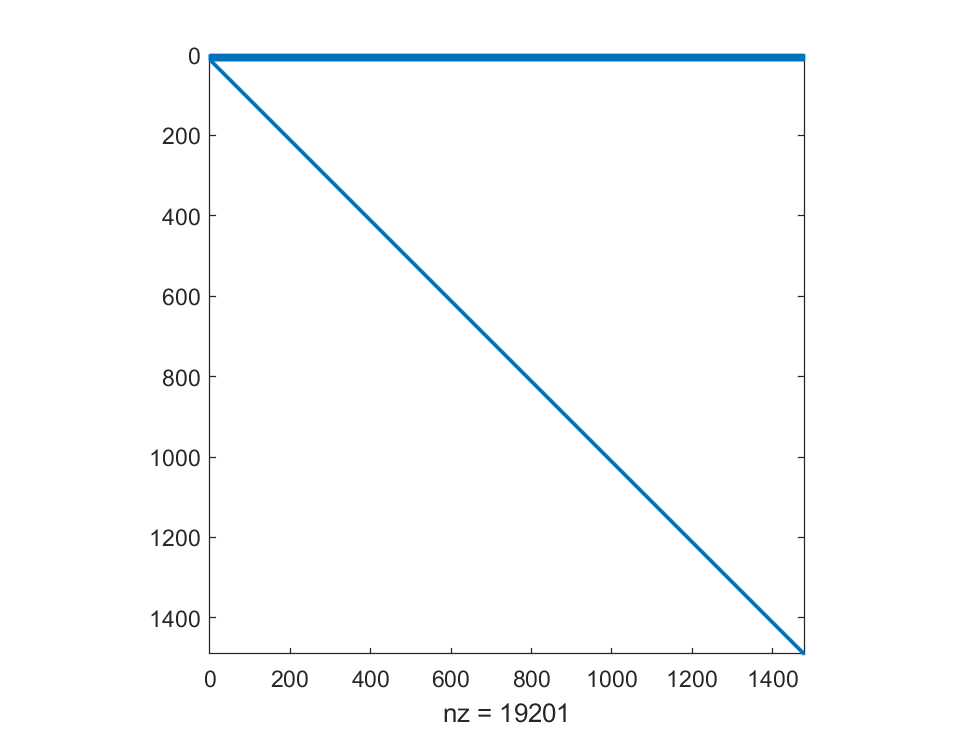
\includegraphics[width = 0.8\linewidth]{images/cg/spy_Xhat.png}
    \caption{Sparsity of $\hat{X}$, $nz$ is the number of non-zero entries.}
    \label{fig:sparsity_x_hat}
\end{figure}

\noindent Now, suppose we wish to perform enough iterations to reduce the norm of the error by a factor of $\epsilon$, that is $\lVert w_{i}-w^*\rVert_A \leq \epsilon \lVert w_{i}-w^*\rVert_A $, then \eqref{eq:cg_rewritten_epsilon} comes at our help suggesting that the maximum number of iterations required from this algorithm is
\begin{equation}
    i \leq \ceil*{\frac{1}{2} \sqrt{\kappa} \log{\left(\frac{2}{\epsilon}\right)}}
    \label{eq:cg_maximum_iterations}
\end{equation}
and we can conclude that the conjugate gradient has a time complexity of $\mathcal{O}(z\sqrt{\kappa})$. This analysis was inspired by the one from Shewchuk et al. \cite{shewchuk1994introduction}.

\subsection{Performance analysis} \label{subsec:cg_performance}

In this section we will take into account the condition number of the matrix $\hat{X}$ rather than the one of $A = \hat{X}^T \hat{X}$ because the CG algorithm \eqref{algorithm:cg} does not explicitly compute it.

\subsubsection{Empirical observation on the execution time}
We know that the algorithm runs in $\mathcal{O}(z\sqrt{\kappa(\hat{X})})$, so we might expect a linear behavior till $\sqrt{\kappa(\hat{X})} < z$. From this point on, the complexity only depends on $\sqrt{\kappa(\hat{X})}$. Unfortunately, this quantity grows exponentially and this implies that when it exceeds the amount of non-zero values of $\hat{X}$, the execution time of the algorithm starts to grow exponentially, as shown in \autoref{fig:cg_plot_conditioning}.

\begin{figure}[H]
    \centering
    \subfloat[Condition number of $\hat{X}$ by varying $\lambda$.]{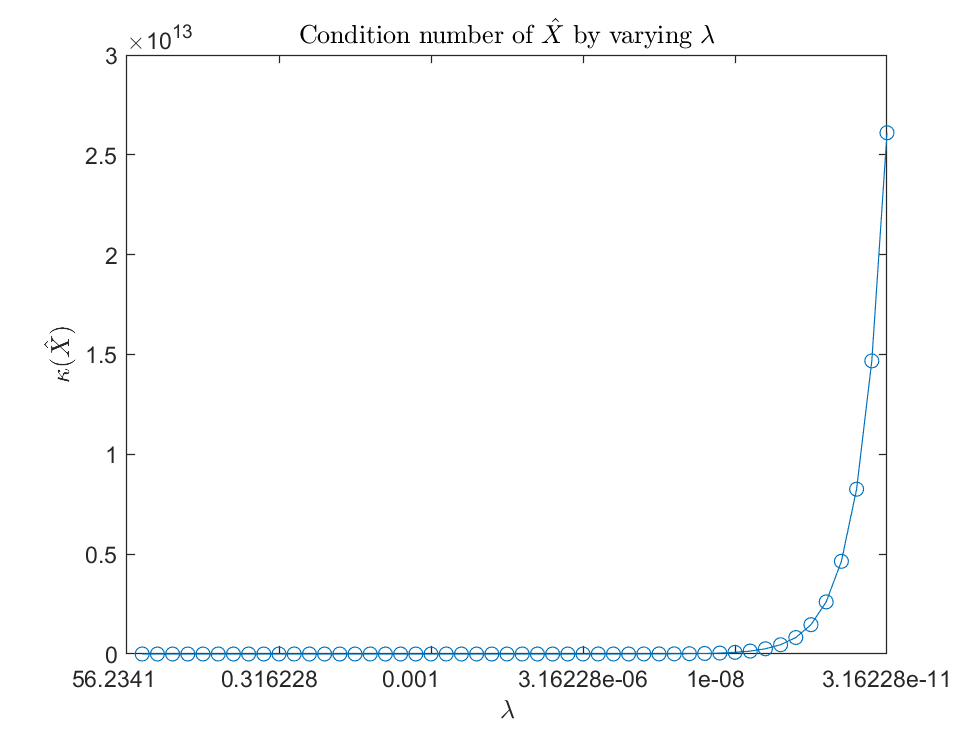
\includegraphics[width=0.62\linewidth]{images/cg/condition_number_X_hat.png}} \\
    \subfloat[Execution time of CG algorithm by varying $\kappa(\hat{X})$.]{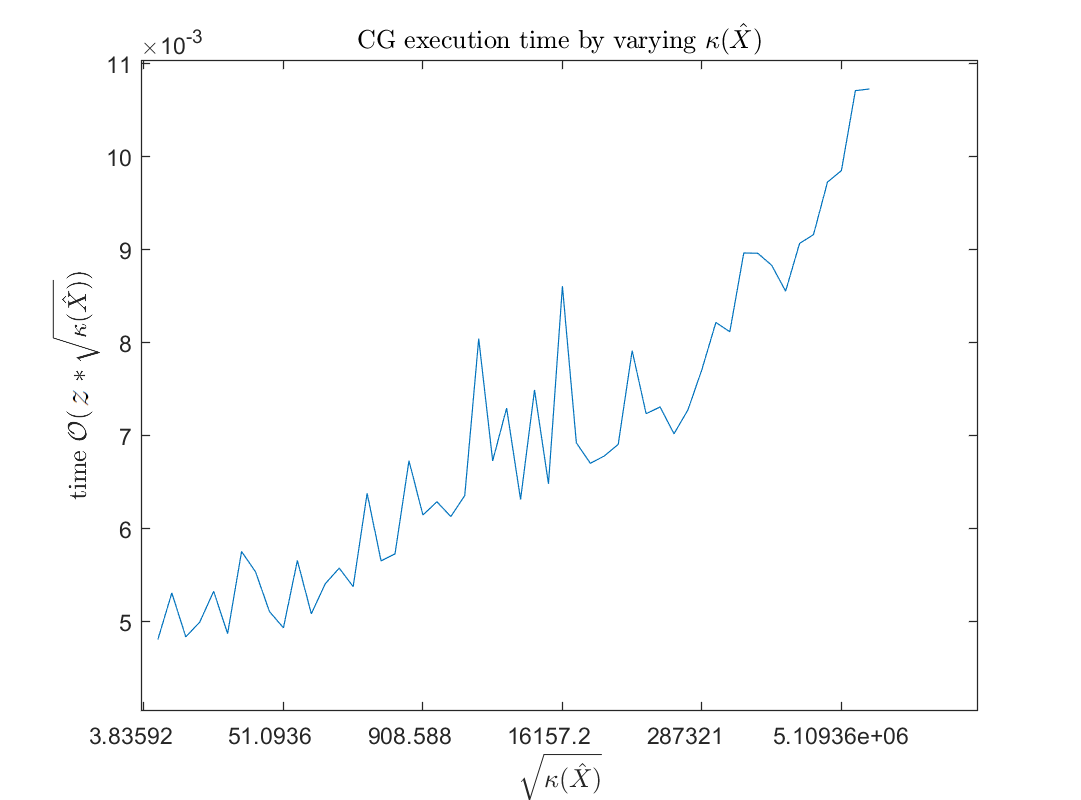
\includegraphics[width=0.62\linewidth]{images/cg/exec_time_cg_cond.png}}
    \caption{Side by side comparison between $\kappa(\hat{X})$ and the execution time of the CG algorithm.}
    \label{fig:cg_plot_conditioning}
\end{figure}

\subsubsection{Superlinear convergence ratio}
By plotting the relative errors $\frac{\lVert w-w^*\rVert}{\lVert w^*\rVert}$ we observed that the conjugate gradient algorithm has a super-linear convergence ratio, this is also confirmed by Beckermann et al. \cite{beckermann2001superlinear}. We decided to show how the conjugate gradient convergence rate changes as $\lambda$ assumes different values, just as we did for the others methods.
\begin{figure}[H]
    \centering
    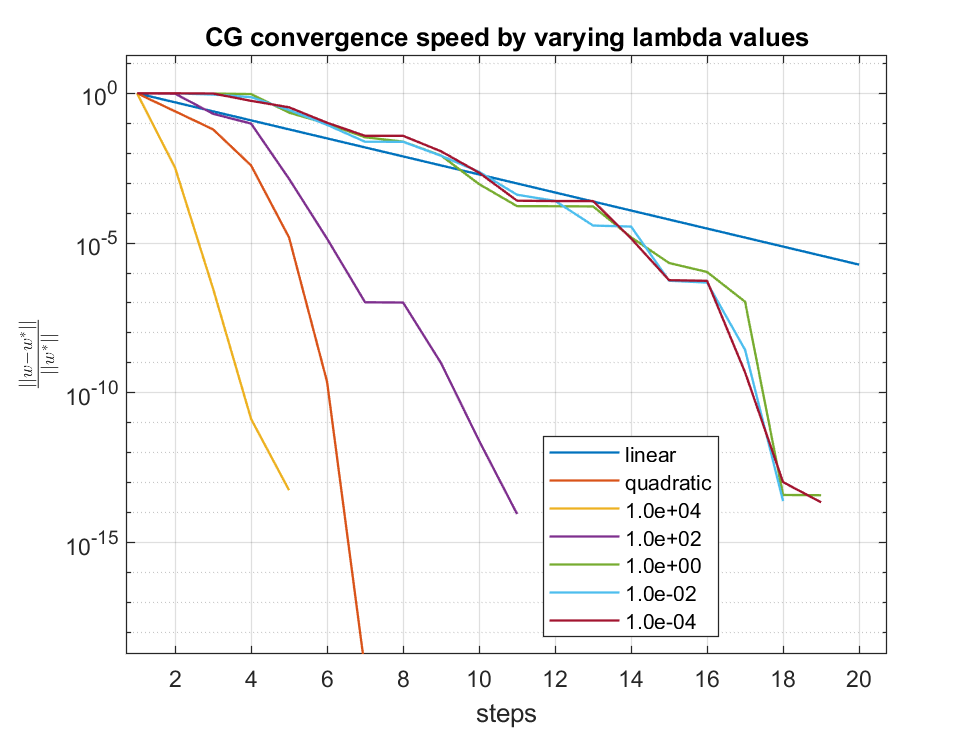
\includegraphics[width = 0.8\linewidth]{images/cg/superlinear_cg.png}
    \caption{CG convergence speed by varying lambdas values.}
    \label{fig:superlinear_cg}
\end{figure}

\noindent As we can see from \autoref{fig:superlinear_cg}, the method reaches a worse convergence ratio as $\lambda$ decreases, like we have seen for L-BFGS.

\subsubsection{Results}
The number of the distinct eigenvalues of $A = \hat{X}^{T} \hat{X}$ is 13, as stated in \ref{appendix:eigenvalues_singular_values}, so we expect to find a solution at most in 13 steps if we were in exact arithmetic as stated by \autoref{theorem:cg_eigenvalues}. As shown in \autoref{tab:cg_results}, CG algorithm found a solution requiring a less number of steps with respect to the theoretical maximum until the matrix $\hat{X}$ is well-conditioned. When $\kappa(\hat{X})$ increases, the algorithm took some more steps to converge. Furthermore, by storing the matrix $\hat{X}$ as sparse, the algorithm runs two order of magnitude faster, doing the same number of iterations. The solution has a relative error of $10^{-14}$ with respect to the Matlab solution $w^* = \hat{X}\backslash \hat{y}$, moreover, we need to point out, again, that using the relative error on $w$ is doable since $w^*$ is unique.
\begin{table}[H]
\centering
\begin{tabular}{c|c|c|c|c} \hline \hline
    $\lambda$&$\frac{\lVert w - w^{*} \lVert}{\rVert w^{*} \lVert}$ & $\frac{\lVert \hat{X}w - y \lVert }{\lVert y \lVert}$ & steps & time (sec)\\ \hline \hline
    
    \rowcolor{gray!30} $10^4$ & $(2.768 \pm 2.726)\times 10^{-14}$ & $ 9.996 \times 10^{-1} \pm 3.268 \times 10^{-4}$ & $4$& $5.5 \times 10^{-4}$\\
    
    $10^2$ & $ 1.477 \times 10^{-14} \pm 5.881 \times 10^{-15}$ & $ 9.336 \times 10^{-1} \pm 4.214 \times 10^{-2}$ & $10$& $1.2 \times 10^{-3}$\\
    
    \rowcolor{gray!30} $1$ & $2.032\times 10^{-14} \pm 4.859 \times 10^{-15} $ & $ 5.606 \times 10^{-2} \pm 6.847 \times 10^{-3} $ & $17$& $1.8 \times 10^{-3}$\\
    
    $10^{-2}$ & $2.754 \times 10^{-14} \pm 4.481 \times 10^{-15}$ & $5.541 \times 10^{-4} \pm 6.994 \times 10^{-5}$ & $17$& $1.9 \times 10^{-3}$\\
    
    \rowcolor{gray!30} $10^{-4}$ & $2.798 \times 10^{-14} \pm 1.002 \times 10^{-15}$ & $5.226 \times 10^{-6} \pm 7.742 \times 10^{-7}$ & $18$ & $2.0 \times 10^{-3}$ \\
    \hline \hline
\end{tabular}
\caption{Conjugate gradient results.}
\label{tab:cg_results}
\end{table}

\noindent The last comparison we did was about the performance of the algorithm with and without explicitly the building of the $A$ matrix. What we noticed is that, in the first case, with the same number of steps, the relative error was one order of magnitude worse than the second one and this happens when the matrix $\hat{X}$ becomes more and more ill-conditioned, that is, when $\lambda < 1$. Moreover, the run time was also an order of magnitude slower.

\begin{table}[H]
\centering
\begin{tabular}{c|c|c|c} \hline \hline
    $\lambda$ & $\frac{\lVert w - w^{*} \lVert}{\rVert w^{*} \lVert}$& $\frac{\lVert w - w^{*} \lVert}{\rVert w^{*} \lVert}$ $A$ explicitly computed & $\frac{\lVert w - w^{*} \lVert}{\rVert w^{*} \lVert}$ Matlab lsqr\\ \hline \hline
    
    \rowcolor{gray!30} $10^4$ & $2.768 \times 10^{-14}$ & $ 1.522 \times 10^{-14}$ & $3.729 \times 10^{-14}$\\
    
    $10^2$ & $ 1.477 \times 10^{-14}$ & $ 2.343 \times 10^{-14}$& $4.206 \times 10^{-14}$\\
    
    \rowcolor{gray!30} $1$ & $2.032\times 10^{-14} $ & $ 3.487 \times 10^{-13} $ & $1.410 \times 10^{-14}$\\
    
    $10^{-2}$ & $2.754 \times 10^{-14}$ & $3.487 \times 10^{-13}$ & $2.051 \times 10^{-14}$\\
    
    \rowcolor{gray!30} $10^{-4}$ & $2.798 \times 10^{-14} $ & $3.605 \times 10^{-13} $ & $1.749 \times 10^{-14}$\\
    \hline \hline
\end{tabular}
\caption{Comparison between the conjugate gradient with and without explicitly computing $A$, the former results are taken from \autoref{tab:cg_results}}.
\label{tab:cg_comparison}
\end{table}

\noindent Comparing our implementation with an off-the-shelf resolver of Matlab, we can state that our implementation works nicely. We first tested our implementation against the \textit{pcg} method (preconditioned conjugate gradient) of matlab without using preconditioning and then versus \textit{lsqr}. The pcg method requires a square matrix in input, so in order to use it we had to explicitly compute $A = \hat{X}^{T} \hat{X}$ and the performance on the errors were almost identical to the ones reported in the third column of \autoref{tab:cg_comparison}. Instead, the lsqr algorithm carried out results close to ours, in terms of relative errors and run time. In order to avoid "verbosity", in \autoref{tab:cg_comparison} we only report the relative errors of this last algorithm.
